\documentclass[11pt]{article}

\usepackage[a4paper, margin=2.5cm]{geometry}
\usepackage[utf8]{inputenc}
\usepackage[T1]{fontenc}
\usepackage{booktabs}
\usepackage{graphicx}
\usepackage{amsmath}
\usepackage{amssymb}
\usepackage{hyperref}
\usepackage{xcolor}
\usepackage{caption}
\usepackage{float}
\usepackage{array}
\usepackage{tikz}
\usetikzlibrary{arrows.meta,positioning,fit,backgrounds,calc}

\hypersetup{
    colorlinks=true,
    linkcolor=blue,
    citecolor=blue,
    urlcolor=blue,
}

\title{MM-MIA: Chest X-Ray Multi-Label Classification \\
\large Image and Text Baselines, and a Q-Former Multimodal Fusion with Cross-Modal Interpretability}
\author{Aziz Chebil \and Hugo Hennion \\ \small Project proj104 -- T\'el\'ecom Paris}
\date{\today}

\begin{document}

\maketitle

\begin{abstract}
This report documents the MM-MIA project: multi-label classification of 21 chest
pathologies from the Open-I chest X-ray dataset~\cite{openi}, approached from three
angles. (1) \emph{Image-only} classifiers (DenseNet-121, ViT) establish a unimodal
visual baseline (mean test AUC 0.73--0.78). (2) \emph{Text-only} classifiers map the
report's indication and findings sections to labels; a TF-IDF + MLP baseline already
reaches a macro AUC of 0.86, and a fine-tuned CXR-BERT~\cite{cxrbert} reaches 0.97,
showing that the textual channel is highly predictive on its own. (3) A
\emph{multimodal} Q-Former~\cite{blip2} (Architecture~3) fuses a frozen CXR-BERT and a
frozen Vision Transformer through learnable label-aligned queries, reaching a macro
test AUC up to 0.984. As an earlier cross-attention fusion model already suggested,
a cross-modal mediation analysis shows that the multimodal gain is largely carried by
text absorbed into the image stream rather than by stronger independent visual
evidence. We therefore study a family of anti-collapse and modality-balancing
mechanisms (pre-norm, modality dropout, an attention-pooled head, and a
gradient-guided modulation, CGGM) that trade a small amount of accuracy for a more
interpretable, less text-dominated model, and we report preliminary unimodal
(indication + image) inference results.
\end{abstract}

\tableofcontents

% ============================================================
\section{Introduction}
% ============================================================

Automated interpretation of chest radiographs is a long-standing benchmark for
medical image analysis, and the public Open-I / Indiana University Chest X-ray
collection~\cite{openi} -- which pairs each radiograph with its free-text radiology
report -- has made it a natural testbed for \emph{multimodal} methods that jointly
exploit pixels and text. The most directly comparable prior work is
TransCheX~\cite{transchex}, a multimodal transformer for chest X-ray classification
that fuses image and report tokens in a single stream; like most report-conditioned
models, it raises the question of how much of its performance comes from the image
versus from the report itself.

This report studies the same Open-I task under three lenses -- image-only, text-only,
and multimodal fusion -- and pays particular attention to \emph{where} a multimodal
model's predictive power actually comes from. We show that the text channel alone is
already strongly predictive, that a Q-Former~\cite{blip2} fusion improves over the
image baselines, and that this improvement is largely mediated by text rather than by
independent visual evidence. We then describe the mechanisms we used to counteract
this text dominance and to make the model more interpretable.

% ============================================================
\section{Task and Dataset}
% ============================================================

The underlying task is multi-label classification of 21 chest conditions
(Atelectasis, Cardiomegaly, Effusion, Pneumonia, Pneumothorax, Edema, Emphysema,
Fibrosis, Infiltration, Mass, Nodule, Hernia, Fracture, Pleural\_Thickening,
Opacity, Consolidation, Granuloma, Calcinosis, Scoliosis, Atherosclerosis, Normal)
from chest radiographs in the Open-I dataset~\cite{openi}. The labeled corpus
contains 7{,}470 paired (image, radiology report) samples; after filtering rows with
empty report text, 6{,}473 samples remain for the multimodal experiments. The label
distribution is heavily imbalanced -- the \emph{Normal} class dominates while classes
such as \emph{Mass} or \emph{Hernia} have only a few dozen positive examples in the
test split (Figure~\ref{fig:dataset}).

\subsection{Structure of the radiology report}

Each Open-I report is semi-structured into free-text sections, of which three are
used here: the \textbf{indication} (the clinical question motivating the exam, e.g.
symptoms or history), the \textbf{findings} (the radiologist's detailed
observations -- the descriptive context), and the \textbf{impression} (the concluding
diagnostic summary, which we treat as the ground-truth read). Table~\ref{tab:report-example}
shows a representative example. This split matters for the rest of the report:
\emph{impression} is used only to derive labels (Section~\ref{sec:label}), while
\emph{indication} and \emph{findings} are the inputs given to the text and multimodal
classifiers.

\begin{table}[H]
\centering
\caption{Example report (Open-I \texttt{CXR2950}) and its three sections.}
\label{tab:report-example}
\renewcommand{\arraystretch}{1.2}
\begin{tabular}{>{\bfseries}p{2.4cm}p{10.5cm}}
\toprule
Section & Text \\
\midrule
Indication & \emph{Allogeneic BMT work-up lab.} \\
Findings   & \emph{The heart is normal in size. The mediastinum is unremarkable.
             The lungs are clear.} \\
Impression & \emph{No acute disease.} $\Rightarrow$ label: \texttt{Normal} \\
\bottomrule
\end{tabular}
\end{table}

% ============================================================
\subsection{Labelisation}
\label{sec:label}
% ============================================================

Labels are derived from the \emph{impression} section only, by rule-based matching of
the National Library of Medicine MeSH terms already indexed for each report in
Open-I~\cite{openi} (\texttt{labeliser.py}). A curated
dictionary (\texttt{MESH\_MAP}) maps each of the 20 pathology classes to a set of MeSH
surface forms (e.g. \emph{cardiomegaly}, \emph{cardiac enlargement}, \emph{enlarged
heart} all map to \texttt{Cardiomegaly}); a case-insensitive substring match assigns
the positive labels, and \texttt{Normal} is set when no pathology fires. Using the
impression rather than the findings avoids feeding the label-bearing text back into
the classifier inputs. The resulting 21-class problem is strongly \emph{uneven}:
\emph{Normal} accounts for the majority of samples, the mid-frequency classes
(\emph{Opacity}, \emph{Calcinosis}, \emph{Granuloma}) have a few hundred positives,
and several findings-level classes (\emph{Mass}, \emph{Pneumothorax},
\emph{Fibrosis}) reach only single-digit positive counts in the test split
(Figure~\ref{fig:dataset}).

\begin{figure}[H]
\centering
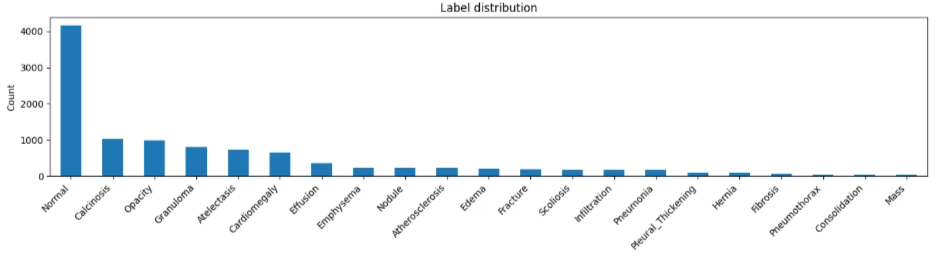
\includegraphics[width=0.85\textwidth]{figures/dataset.png}
\caption{Label distribution over the 21 classes (heavily imbalanced).}
\label{fig:dataset}
\end{figure}

% ============================================================
\section{Image Classification Models}
\label{sec:cv}
% ============================================================

Two image-only architectures were trained and evaluated, all under the same
multi-label AUC-ROC evaluation protocol.

\subsection{Model 1 -- DenseNet-121 baseline (\texttt{cv\_model\_01.ipynb})}

\textbf{Architecture.} An ImageNet-pretrained DenseNet-121 backbone with a custom
classification head: \texttt{Linear(1024$\to$512) $\to$ ReLU $\to$ Dropout(0.5)
$\to$ Linear(512$\to$21)}.

\textbf{Training setup.}
\begin{itemize}
  \item Loss: \texttt{BCEWithLogitsLoss} with per-class positive weights to
        counteract label imbalance.
  \item Optimizer: AdamW, lr $=10^{-4}$, weight decay $=10^{-4}$, cosine annealing
        schedule.
  \item Image size $224\times224$, batch size 32, max 20 epochs, early stopping
        patience 5.
  \item Augmentations: horizontal flip, rotation $\pm15^\circ$, random affine
        translation, color jitter.
  \item Backbone trained fully from the start (no freezing phase).
\end{itemize}

Training stopped early at epoch 17. Best validation AUC was 0.7787 (epoch 12);
final test mean AUC was \textbf{0.7802}.

\begin{table}[H]
\centering
\caption{DenseNet-121 -- per-class test AUC-ROC.}
\begin{tabular}{lc}
\toprule
Condition & AUC-ROC \\
\midrule
Emphysema           & 0.9419 \\
Hernia              & 0.9277 \\
Consolidation       & 0.9164 \\
Cardiomegaly        & 0.8849 \\
Effusion            & 0.8677 \\
Edema               & 0.8581 \\
Atelectasis         & 0.8217 \\
Atherosclerosis     & 0.8196 \\
Opacity             & 0.8104 \\
Infiltration        & 0.8063 \\
Fibrosis            & 0.7934 \\
Pneumothorax        & 0.7858 \\
Mass                & 0.7692 \\
Pneumonia           & 0.7680 \\
Normal              & 0.7577 \\
Pleural\_Thickening & 0.7514 \\
Calcinosis          & 0.6748 \\
Granuloma           & 0.6719 \\
Fracture            & 0.6346 \\
Nodule              & 0.5903 \\
Scoliosis           & 0.5320 \\
\midrule
\textbf{Mean AUC}   & \textbf{0.7802} \\
\bottomrule
\end{tabular}
\end{table}

\begin{figure}[H]
\centering
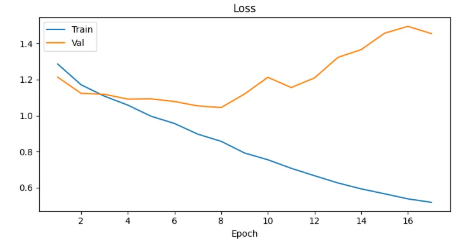
\includegraphics[width=0.6\textwidth]{figures/densenet_loss_func.png}
\caption{DenseNet-121 -- training and validation loss curves.}
\label{fig:densenet-loss}
\end{figure}

\subsection{Model 2 -- ViT (\texttt{cv\_model\_vit\_04.ipynb})}

Fine-tuned the following open-source model: `https://huggingface.co/codewithdark/vit-chest-xray`


\textbf{Loss change -- Asymmetric Loss (ASL).} This loss function allowed us to focus on the different classes we have in the dataset and put coefficients proportionally to the number of the class samples in the dataset.

\textbf{Stronger augmentations.} \texttt{RandomAffine} (translation, scale, shear,
simulating patient positioning variance), \texttt{ElasticTransform} (soft-tissue
deformation), \texttt{RandomErasing} (simulating occlusions/implants), and a
broadened \texttt{ColorJitter} range.

\textbf{Training setup.} AdamW with a 3-epoch linear warmup ($5\times10^{-6} \to
5\times10^{-5}$) followed by cosine decay to $10^{-6}$; backbone frozen during
warmup and unfrozen at epoch 4 with $\text{lr}=5\times10^{-6}$; batch size 16; up
to 30 epochs with early-stopping patience 7.

\textbf{Results.} Best validation AUC reached 0.7885 (epoch 23); final test mean
AUC was \textbf{0.7330}. Table~\ref{tab:vit-v4} compares per-class AUC against the
ViT v3 reference run used during development.

\begin{table}[H]
\centering
\caption{ViT AUC results}
\label{tab:vit-v4}
\begin{tabular}{lccc}
\toprule
Condition & AUC  \\
\midrule
Fibrosis            & 0.907 \\
Emphysema           & 0.877 \\
Effusion            & 0.87 \\
Hernia              & 0.86 \\
Cardiomegaly        & 0.862 \\
Edema               & 0.84 \\
Consolidation       & 0.845 \\
Atherosclerosis     & 0.767 \\
Opacity             & 0.75 \\
Atelectasis         & 0.740 \\
Pneumothorax        & 0.728 \\
Normal              & 0.723  \\
Pneumonia           & 0.677  \\
Infiltration        & 0.675  \\
Scoliosis           & 0.639  \\
Calcinosis          & 0.636  \\
Pleural\_Thickening & 0.627  \\
Mass                & 0.607  \\
Nodule              & 0.601  \\
Granuloma           & 0.582  \\
Fracture            & 0.557  \\
\bottomrule
\end{tabular}
\end{table}

\begin{figure}[H]
\centering
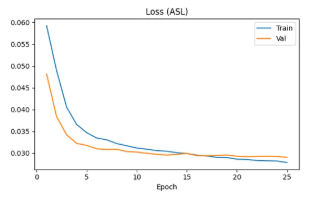
\includegraphics[width=0.55\textwidth]{figures/ViT_final_loss_func.png}
\caption{ViT v4 -- training and validation loss curves (Asymmetric Loss).}
\label{fig:vit-loss}
\end{figure}

% ============================================================
\section{Text Classification}
\label{sec:text}
% ============================================================

The image models above plateau around 0.73--0.78 mean AUC. Before fusing modalities,
we ask how far the \emph{text} alone goes. The task is identical -- predict the 21
labels -- but the input is now the report's \emph{indication} + \emph{findings}
sections concatenated (the label-bearing \emph{impression} is excluded).

\subsection{TF-IDF + MLP baseline}

A deliberately simple baseline vectorises indication and findings with two TF-IDF
encoders ($\sim$1{,}400 features after \texttt{min\_df} filtering) and feeds them to a
small multi-layer perceptron (\texttt{Linear(1432$\to$64) $\to$ ReLU $\to$
Dropout(0.3) $\to$ Linear(64$\to$21)}) trained with a positive-weighted
\texttt{BCEWithLogitsLoss}. Despite its simplicity it already reaches a macro test
AUC of \textbf{0.864} and a micro AUC of \textbf{0.927} (Figure~\ref{fig:mlp}).

\begin{figure}[H]
\centering
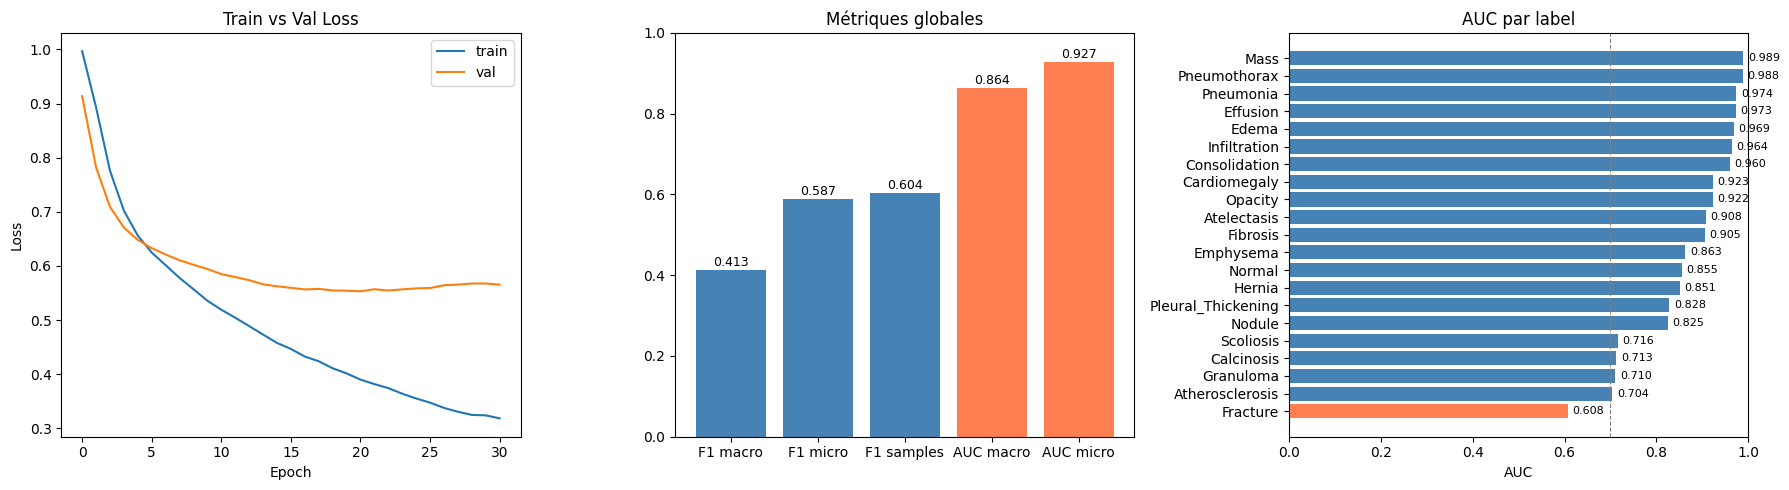
\includegraphics[width=\textwidth]{figures/mlp_tfidf_perf.png}
\caption{TF-IDF + MLP text baseline -- training curves, global metrics, and per-label
test AUC. A bag-of-words model already separates most labels.}
\label{fig:mlp}
\end{figure}

That such a shallow model performs this well indicates the task is, in large part,
\emph{easy from text}: the \emph{indication} field alone often names or strongly
implies the pathology, so much of the label signal is carried lexically. This is the
same effect that makes report-conditioned models such as TransCheX~\cite{transchex}
strong, and it foreshadows the text-dominance we quantify for the multimodal model in
Section~\ref{sec:interp} and~\ref{sec:qexplain}.

\subsection{CXR-BERT-specialized}

To exploit the medical language properly we fine-tune
\texttt{microsoft/BiomedVLP-CXR-BERT-specialized}~\cite{cxrbert}, a BERT pre-trained on
radiology text, with a linear classification head over the \texttt{[CLS]} token. We
use progressive unfreezing (head only for the first epoch, then the top two
transformer layers), AdamW (lr $2\times10^{-5}$), and threshold selection on the
validation set. On the full 21-label test set it reaches a macro AUC of
\textbf{0.972}, a micro AUC of \textbf{0.987}, and a macro F1 of \textbf{0.734}
(Figure~\ref{fig:cxrbert}) -- a large gain over the bag-of-words baseline and far
above any image-only model.

\begin{figure}[H]
\centering
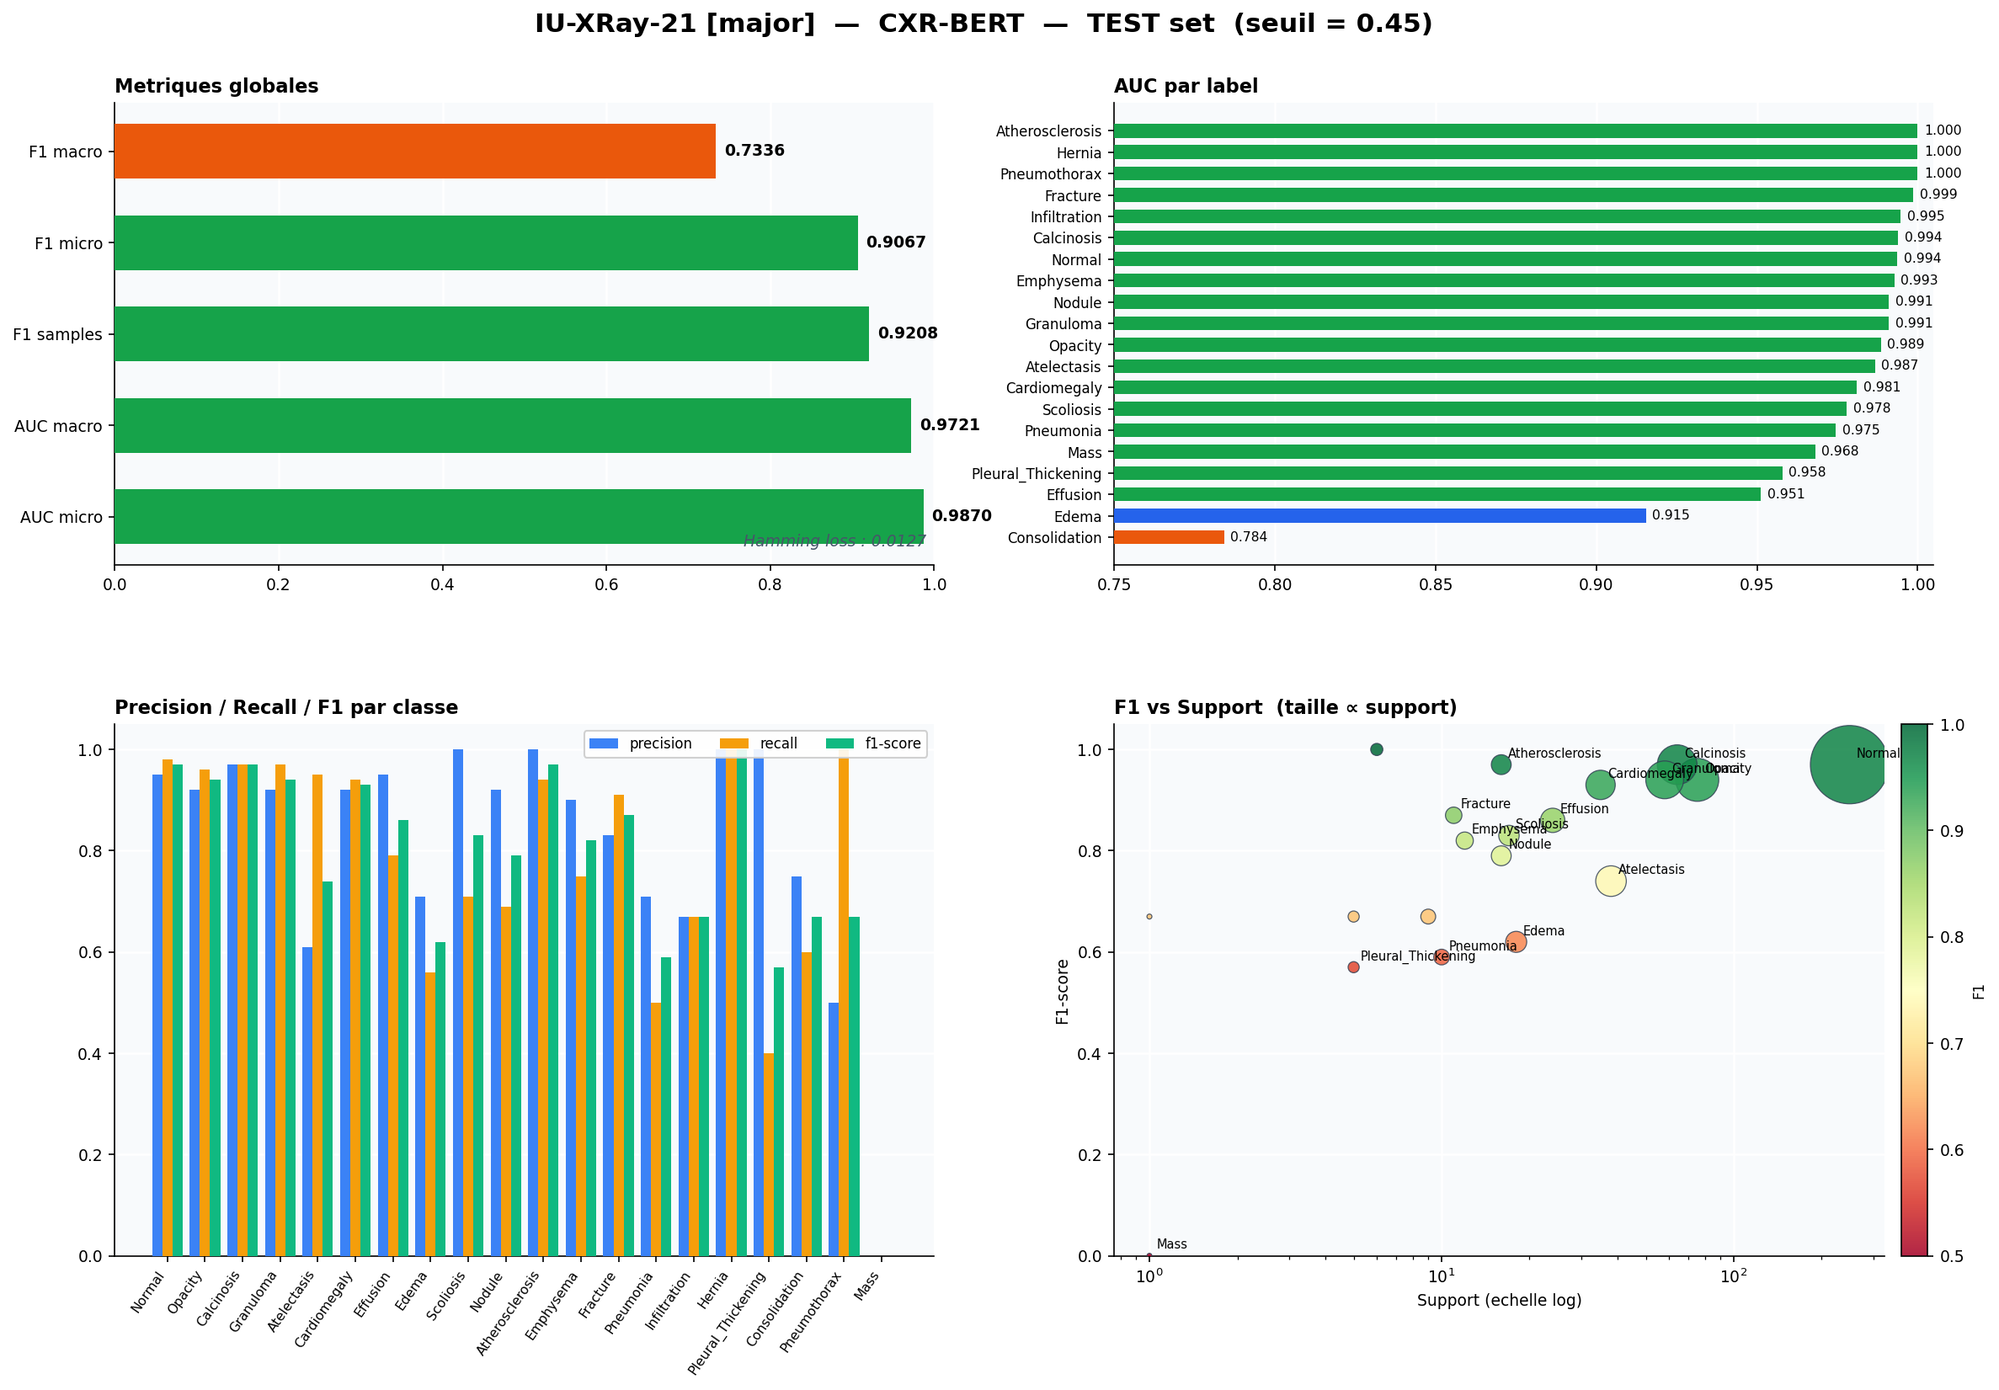
\includegraphics[width=\textwidth]{figures/cxrbert_test.png}
\caption{CXR-BERT-specialized -- IU-XRay 21-label test set. Global metrics (left),
per-label AUC (right), per-class precision/recall/F1 and F1-vs-support (bottom).}
\label{fig:cxrbert}
\end{figure}

\begin{table}[H]
\centering
\caption{Text vs.\ image: mean test AUC by modality.}
\label{tab:text-vs-image}
\begin{tabular}{llc}
\toprule
Modality & Model & Macro AUC \\
\midrule
Image & DenseNet-121          & 0.780 \\
Image & ViT (chest-xray)      & 0.733 \\
Text  & TF-IDF + MLP          & 0.864 \\
Text  & CXR-BERT-specialized  & \textbf{0.972} \\
\bottomrule
\end{tabular}
\end{table}

% ============================================================
\section{Multimodal Fusion -- Architecture 1}
\label{sec:fusion}
% ============================================================

\subsection{Architecture}

The fusion model (\texttt{multimodal\_fusion/architecture\_1/model.py}) combines a
custom BERT-style text encoder and the same pretrained ViT image encoder via
\textbf{bidirectional cross-attention}.

\begin{table}[H]
\centering
\caption{MultimodalFusion architecture components.}
\begin{tabular}{ll}
\toprule
Component & Details \\
\midrule
Text encoder & Custom BERT - 4.3M params \\
Image encoder & \texttt{codewithdark/vit-chest-xray} ViT-B/16 (d=768, 197 tokens) -- 86M params \\
Cross-attention & Bidirectional, 8 heads, $d_{\text{model}}=512$ \\
Text pooling & \texttt{[CLS]} token of fused text sequence \\
Image pooling & Learned soft-attention over all 197 fused image tokens \\
Classification head & Linear(1024$\to$512) + LayerNorm + GELU + Dropout + Linear(512$\to$21) \\
\textbf{Total parameters} & \textbf{95{,}931{,}925} \\
\bottomrule
\end{tabular}
\end{table}

Both modalities are first projected to a common space ($d=512$):
text tokens $(B,L,256) \to (B,L,512)$ and image tokens $(B,197,768) \to
(B,197,512)$. Two cross-attention directions are then computed in parallel on
these projections:
\begin{itemize}
  \item \textbf{Text$\to$Image (t2i):} text tokens as queries, image tokens as
        keys/values -- text representations are enriched with visual context.
  \item \textbf{Image$\to$Text (i2t):} image tokens as queries, text tokens as
        keys/values -- image representations are enriched with textual context.
\end{itemize}
Each branch then passes through a residual connection, an FFN
($512\to1024\to512$), and LayerNorm. The pooled text representation
(\texttt{[CLS]} of the fused text sequence) is concatenated with the pooled image
representation (learned attention pooling over all 197 fused image tokens) and fed
to the classification head.

\subsection{Dataset and Training}



\begin{table}[H]
\centering
\caption{Two-phase training schedule.}
\begin{tabular}{lccc}
\toprule
Phase & Epochs & Trainable parameters & Learning rate \\
\midrule
1 & 1--3  & Cross-attention + head only (5.3M) & Warmup $5\times10^{-6} \to 5\times10^{-5}$ \\
2 & 4--30 & All parameters (95.9M) & Head $5\times10^{-5}$, backbone $5\times10^{-6}$, cosine $\to 10^{-6}$ \\
\bottomrule
\end{tabular}
\end{table}


\subsection{Results}

\begin{table}[H]
\centering
\caption{Fusion model training curve (key epochs).}
\begin{tabular}{lll}
\toprule
Epoch & Phase & Val AUC \\
\midrule
1  & Frozen   & 0.6247 \\
3  & Frozen   & 0.9206 \\
4  & Unfrozen & 0.9596 \\
8  & Unfrozen & 0.9879 $\star$ \\
15 & Unfrozen & 0.9881 $\star$ (best) \\
22 & Unfrozen & early stop \\
\bottomrule
\end{tabular}
\end{table}

\begin{table}[H]
\centering
\caption{Fusion model -- per-class test AUC (968 samples).}
\begin{tabular}{lc}
\toprule
Pathology & AUC \\
\midrule
Atelectasis         & 0.9875 \\
Cardiomegaly        & 0.9887 \\
Effusion            & 0.9731 \\
Pneumonia           & 0.9670 \\
Pneumothorax        & 0.9969 \\
Edema               & 0.9922 \\
Emphysema           & 0.9604 \\
Fibrosis            & 0.9550 \\
Infiltration        & 0.9839 \\
Mass                & 0.9946 \\
Nodule              & 0.9918 \\
Hernia              & 0.9997 \\
Fracture            & 0.9922 \\
Pleural\_Thickening & 1.0000 \\
Opacity             & 0.9999 \\
Consolidation       & 0.9936 \\
Granuloma           & 0.9999 \\
Calcinosis          & 0.9974 \\
Scoliosis           & 0.9950 \\
Atherosclerosis     & 1.0000 \\
Normal              & 0.9920 \\
\midrule
\textbf{Mean AUC}   & \textbf{0.9886} \\
\bottomrule
\end{tabular}
\end{table}

\begin{figure}[H]
\centering
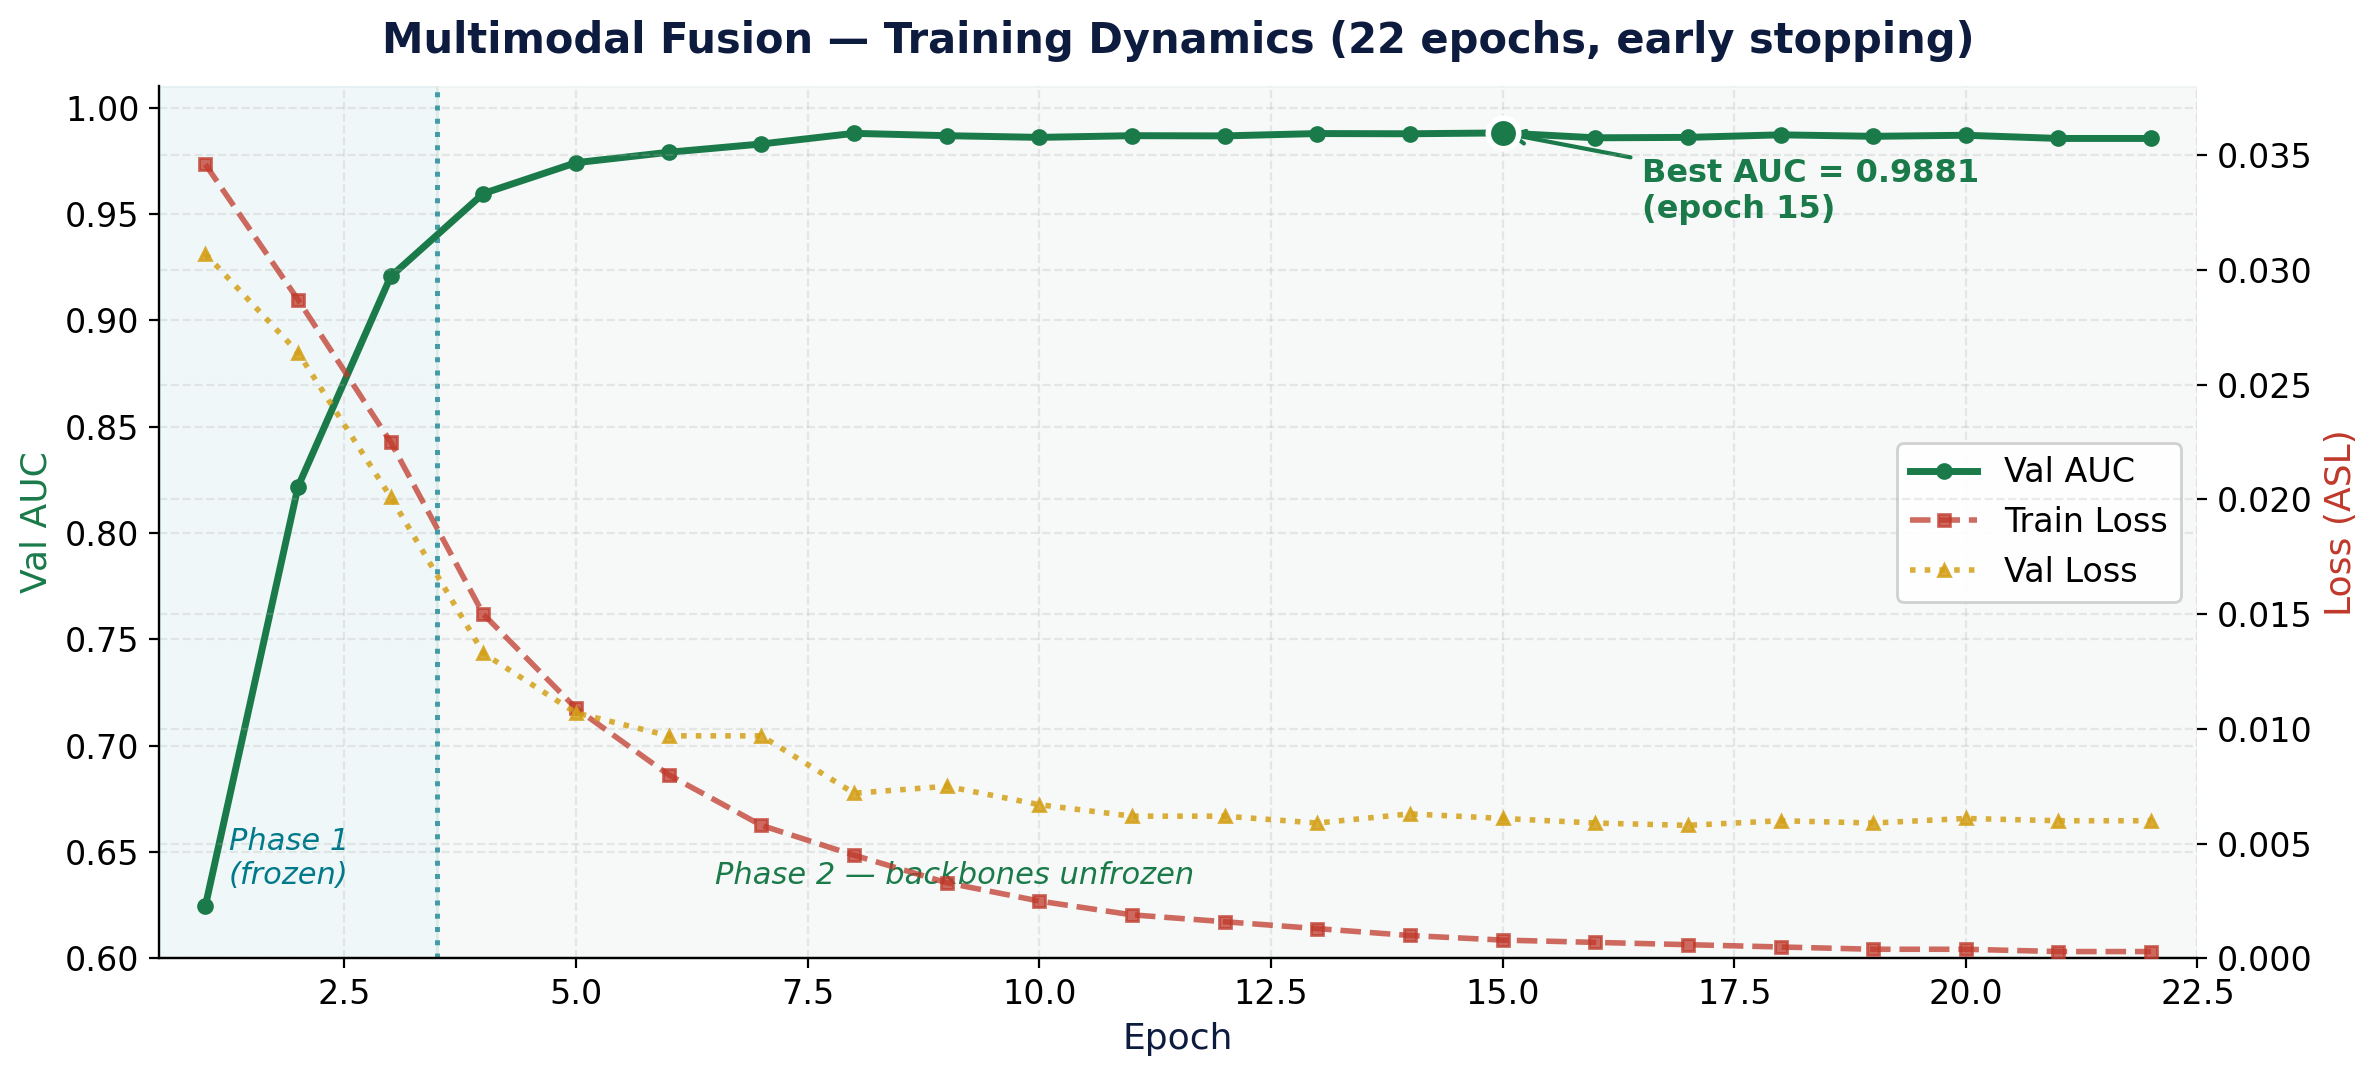
\includegraphics[width=0.75\textwidth]{figures/fig3_training_curve_multi_modal.png}
\caption{Multimodal fusion model -- training/validation loss and validation AUC
across the two-phase training schedule.}
\label{fig:fusion-loss}
\end{figure}

The fusion model's mean test AUC (\textbf{0.9886}) is roughly 0.21--0.26 higher than
any image-only model from Section~\ref{sec:cv} (which plateau around
0.73--0.78). Such a large jump from adding text input is itself the motivation for
the interpretability investigation in the next section: is this gain explained by
the model learning to combine complementary visual and textual evidence, or by a
narrower, less desirable mechanism?

% ============================================================
\section{Interpretability Analysis}
\label{sec:interp}
% ============================================================

Two complementary interpretability techniques were applied to the fusion model:
attention visualization (qualitative, image-focused), and a full test-set
cross-modal mediation analysis with AUC-based metrics (quantitative, all 21
labels), informed along the way by a single-sample text counterfactual probe.
Together they build toward the central finding of this report.

\subsection{Attention Heatmaps}

Visualizing the learned image-pooling attention weights and Image$\to$Text
cross-attention maps shows some variation across pathologies, but several
high-attention regions fall near image borders or outside clinically relevant
anatomy:

\begin{itemize}
  \item \textbf{Pneumothorax:} strongest attention near the left image border,
        partially outside the lung field -- not anatomically consistent with
        typical pneumothorax presentation.
  \item \textbf{Cardiomegaly:} attention spread across lower thoracic regions,
        without clearly emphasizing the cardiac silhouette.
  \item \textbf{Effusion:} attention pattern differs from frontal-view cases,
        loosely overlapping lower thoracic areas where pleural effusions are
        commonly observed, but remaining diffuse.
  \item \textbf{Normal:} multiple hotspots despite the absence of pathology,
        including border regions, with no specific anatomical correspondence.
\end{itemize}

\begin{figure}[H]
\centering
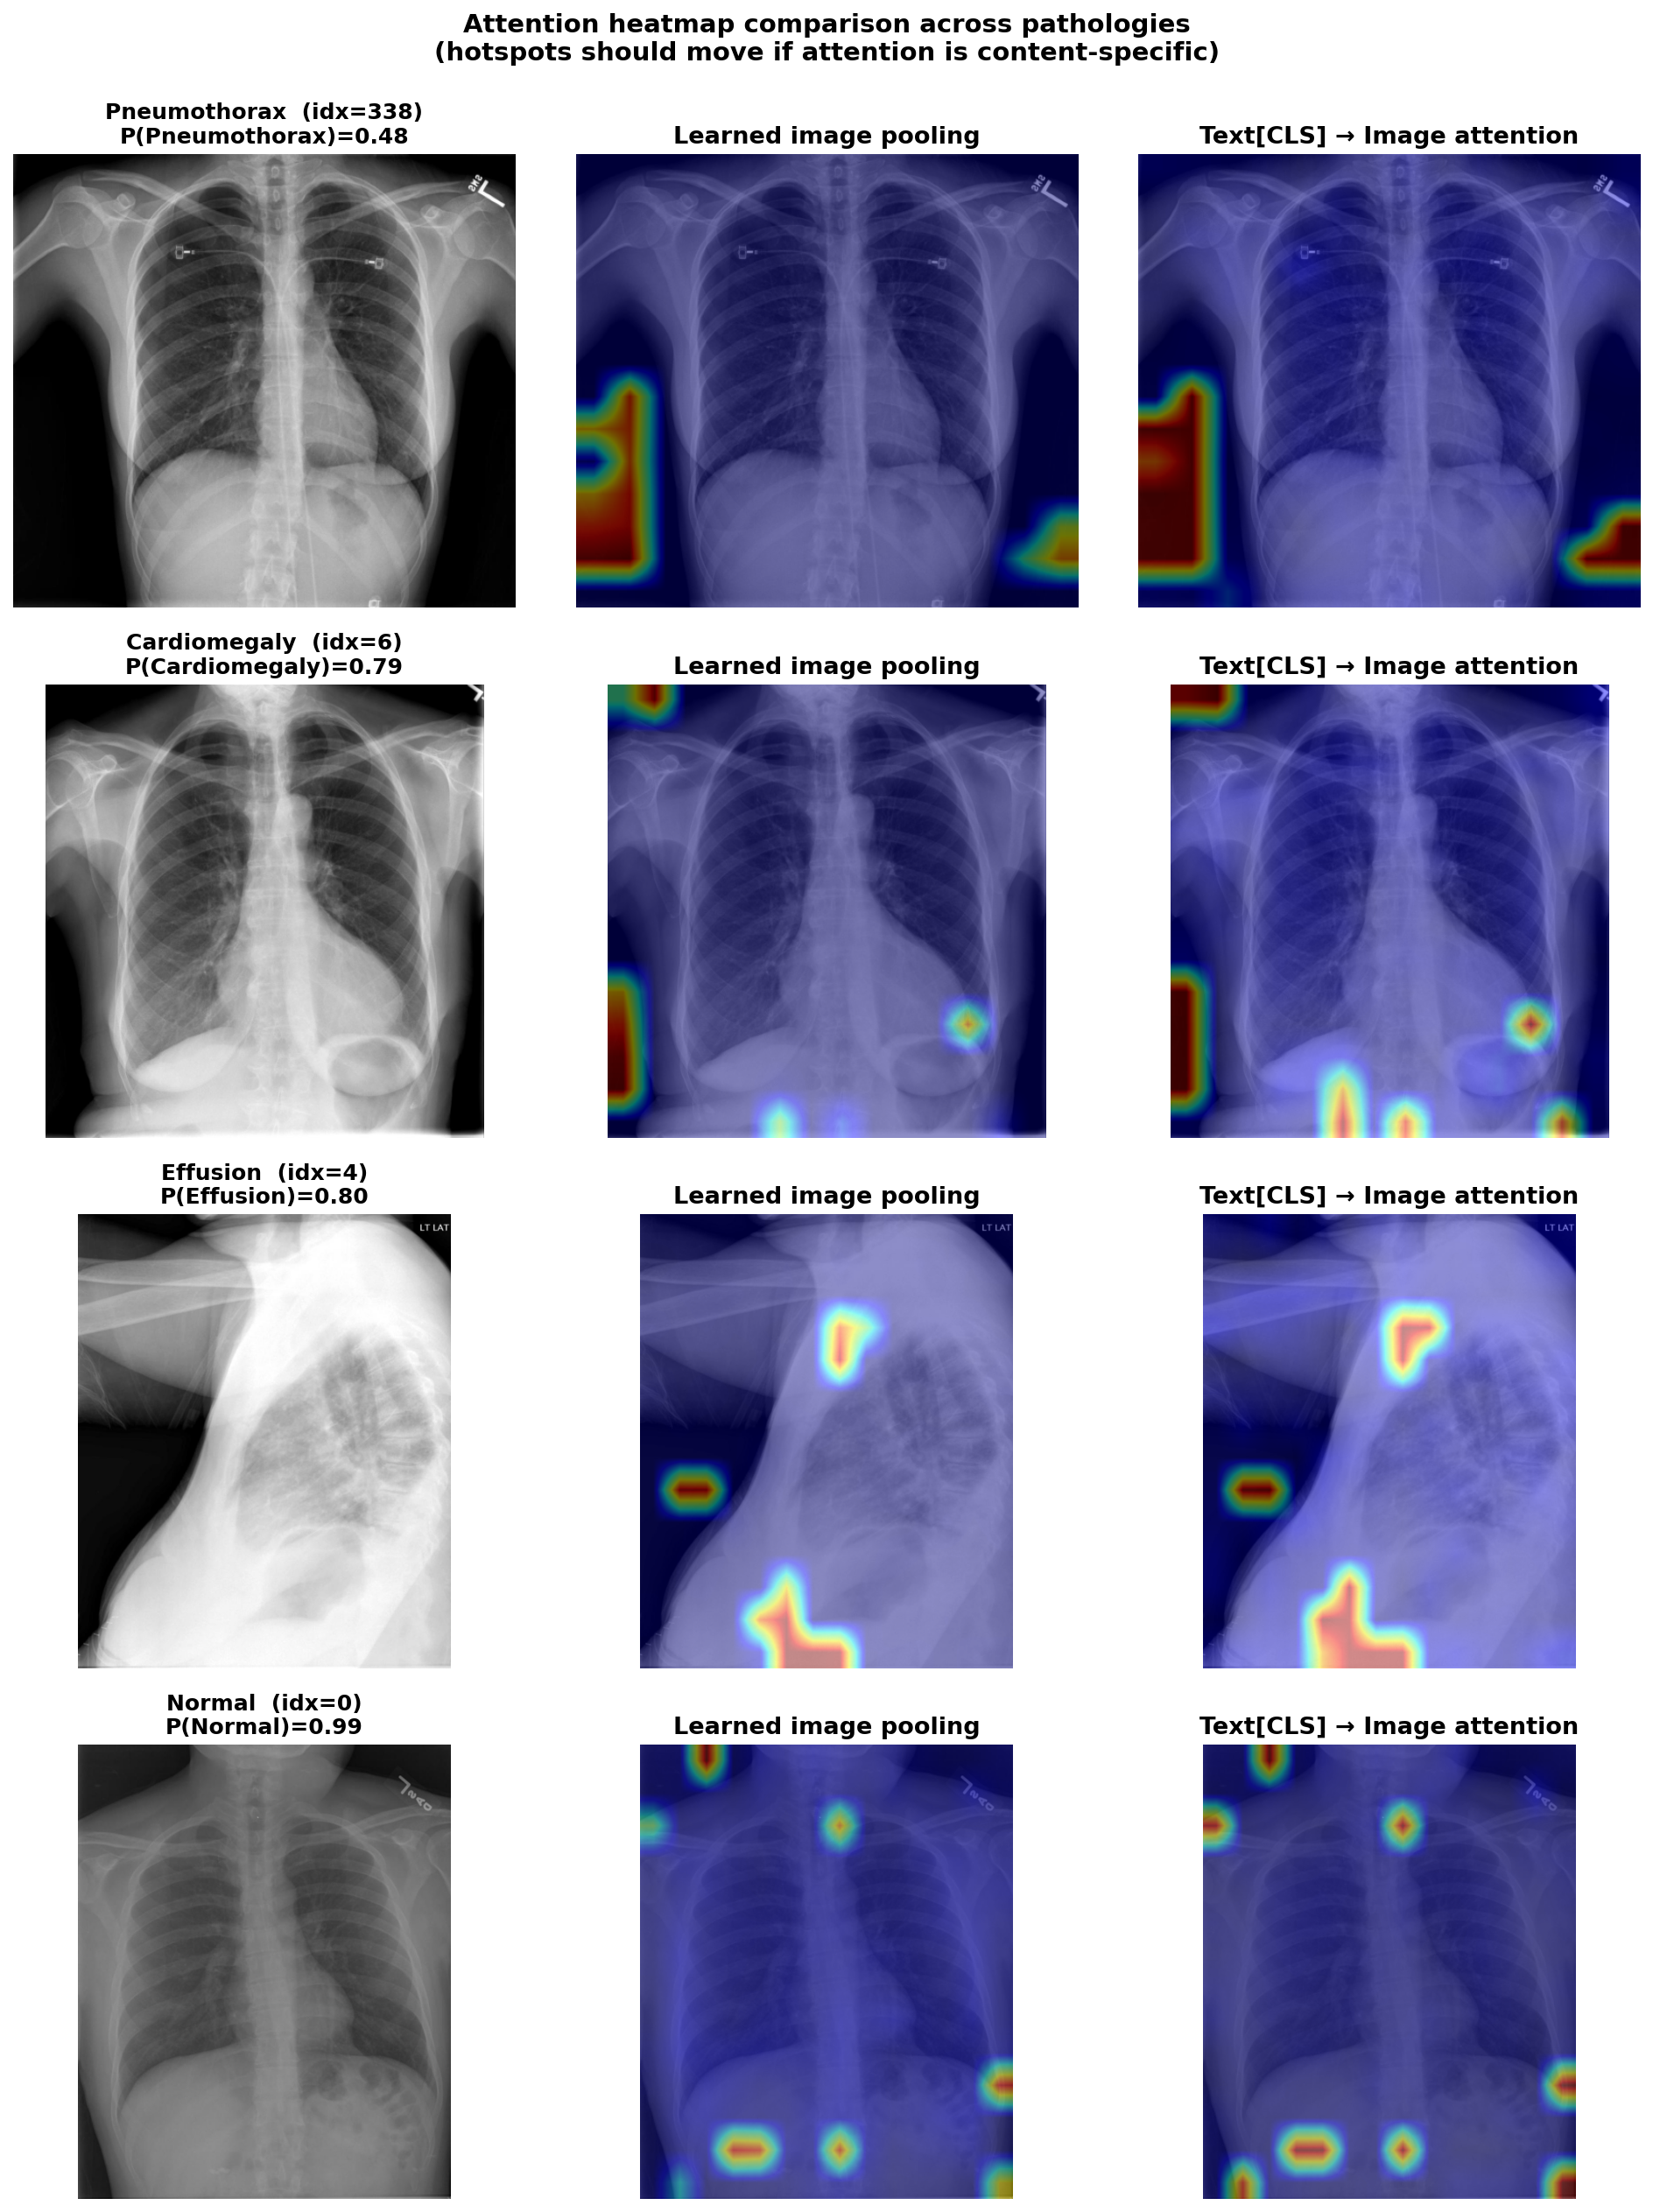
\includegraphics[width=0.6\textwidth]{figures/attention_comparaison.png}
\caption{Attention heatmap comparison across pathologies}
\label{fig:attention}
\end{figure}



\subsection{Cross-Modal Mediation Analysis}

\subsubsection{Method}

For a given sample, the model is run twice through the shared backbone: once with
the real radiology report, once with blank text. This produces two representation
pairs, $(\text{text}_R, \text{image}_R)$ and $(\text{text}_B, \text{image}_B)$,
where the subscripts $R$/$B$ denote ``real text'' and ``blank text'' forward
passes respectively. These pooled representations are then recombined and passed
through the shared classification head, isolating each branch's contribution:

\begin{itemize}
  \item \textbf{real\_real} $= (\text{text}_R, \text{image}_R)$: the full model,
        reproducing the reported test AUC.
  \item \textbf{blankT+realI} $= (\text{text}_B, \text{image}_R)$: discards the
        text representation but keeps the image representation \emph{as it was
        produced during a forward pass that did see the real report} (i.e., after
        being shaped by Image$\to$Text cross-attention).
  \item \textbf{realT+blankI} $= (\text{text}_R, \text{image}_B)$: discards the
        image representation but keeps the text representation, paired with an
        image representation that never saw real text content.
\end{itemize}

An initial version of this experiment (\texttt{representation\_mediation.py})
averaged mean predicted probability over $n=30$ positive samples for 4
pathologies. To make the analysis rigorous, it was extended
(\texttt{mediation\_auc.py}) to the \textbf{full 968-sample test set and all 21
labels}, replacing mean probability with \textbf{ROC-AUC} per condition -- a
ranking-based metric that is insensitive to a uniform shift in predicted
probability and therefore directly measures whether each condition still
discriminates positive from negative samples.

\subsubsection{Results}

\begin{table}[H]
\centering
\small
\caption{Cross-modal mediation analysis -- full test set ($n=968$), AUC per
condition and per pathology. $\Delta = \text{AUC(real\_real)} -
\text{AUC(blankT+realI)}$.}
\begin{tabular}{lccccc}
\toprule
Pathology & $n_{\text{pos}}$ & AUC real & AUC blankT+realI & AUC realT+blankI & $\Delta$ \\
\midrule
Atelectasis         & 93  & 0.9825 & 0.9858 & 0.6512 & $-0.0033$ \\
Cardiomegaly        & 82  & 0.9817 & 0.9844 & 0.9286 & $-0.0027$ \\
Effusion            & 41  & 0.9758 & 0.9723 & 0.8736 & $+0.0035$ \\
Pneumonia           & 22  & 0.9681 & 0.9435 & 0.6647 & $+0.0246$ \\
Pneumothorax        & 6   & 0.9977 & 0.9971 & 0.9182 & $+0.0007$ \\
Edema               & 25  & 0.9506 & 0.9703 & 0.8780 & $-0.0197$ \\
Emphysema           & 32  & 0.9494 & 0.9576 & 0.8571 & $-0.0082$ \\
Fibrosis            & 6   & 0.9463 & 0.9539 & 0.8557 & $-0.0076$ \\
Infiltration        & 19  & 0.9685 & 0.9612 & 0.7677 & $+0.0073$ \\
Mass                & 5   & 0.9915 & 0.9668 & 0.8546 & $+0.0247$ \\
Nodule              & 28  & 0.9894 & 0.9938 & 0.6169 & $-0.0044$ \\
Hernia              & 12  & 0.9997 & 0.9994 & 0.7494 & $+0.0003$ \\
Fracture            & 27  & 0.9831 & 0.9959 & 0.7204 & $-0.0128$ \\
Pleural\_Thickening & 13  & 0.9998 & 0.9989 & 0.7729 & $+0.0010$ \\
Opacity             & 132 & 0.9996 & 0.9988 & 0.6720 & $+0.0008$ \\
Consolidation       & 7   & 0.9915 & 0.9917 & 0.8910 & $-0.0001$ \\
Granuloma           & 105 & 0.9999 & 0.9997 & 0.5967 & $+0.0002$ \\
Calcinosis          & 129 & 0.9954 & 0.9930 & 0.6368 & $+0.0024$ \\
Scoliosis           & 24  & 0.9916 & 0.9802 & 0.7138 & $+0.0113$ \\
Atherosclerosis     & 33  & 1.0000 & 1.0000 & 0.7466 & $0.0000$ \\
Normal              & 553 & 0.9876 & 0.9853 & 0.6951 & $+0.0022$ \\
\midrule
\textbf{Mean}       & --  & \textbf{0.9833} & \textbf{0.9824} & \textbf{0.7648} & \textbf{0.0010} \\
\bottomrule
\end{tabular}
\end{table}


\subsubsection{Interpretation}

Removing the text input while keeping an image representation that did see the real report costs essentially zero AUC, and is slightly negative for seven of 21 pathologies. The text representation alone (realT+blankI) is weaker (mean AUC 0.76480) -- above chance, so reports carry real signal, but secondary to whatever produces the near-perfect blankT+realI AUC.
We can conlcude that the image representation with the text2image signal carries the most information used by the model to predict the relevant pathology.

% ============================================================
\section{Multimodal Fusion -- Architecture 3 (Q-Former)}
\label{sec:qformer}
% ============================================================

Architecture~1 fuses the two streams symmetrically, which makes it hard to control
the text dominance highlighted in Section~\ref{sec:interp}. Architecture~3 takes the
opposite, asymmetric stance inspired by the Q-Former of BLIP-2~\cite{blip2}: both
encoders are \emph{frozen}, and a small set of learnable \emph{queries} -- one per
label -- distils evidence from the image while being conditioned on the text. Only
the queries and the head are trained ($\sim$28--31\,M trainable parameters out of
$\sim$225\,M), which keeps the visual and textual representations fixed and isolates
\emph{how} the two are combined. These experiments use the 14-label NIH subset
(\texttt{--mode 14}).

\subsection{Architecture}

The text (indication + findings) is encoded by the frozen
CXR-BERT~\cite{cxrbert} into token features $T\in\mathbb{R}^{B\times L\times 768}$, and
the radiograph by the frozen ViT~\cite{vit} \texttt{codewithdark/vit-chest-xray} into
patch tokens $Z\in\mathbb{R}^{B\times 197\times 768}$. A bank of $14$ learnable queries
$Q$ is passed through three \emph{Joint Query Blocks}; each block (i) applies
self-attention over the concatenation $[Q;T]$ (only the queries are updated, so they
read the text), (ii) applies cross-attention from $Q$ to the image tokens $Z$, and
(iii) applies a position-wise FFN, all with residual connections. The output queries
$q_j$ feed a \emph{diagonal, label-aligned} head, $\text{logit}_j = w_j\!\cdot\! q_j +
b_j$, so that query $j$ -- and its attention map -- is responsible for exactly
pathology $j$. We compare two ways of feeding text to the blocks.

\paragraph{``last'' variant.} All three blocks read the \emph{final} CXR-BERT hidden
layer (Figure~\ref{fig:qf-last}). The text is encoded once and reused.

\begin{figure}[H]
\centering
\resizebox{\textwidth}{!}{%
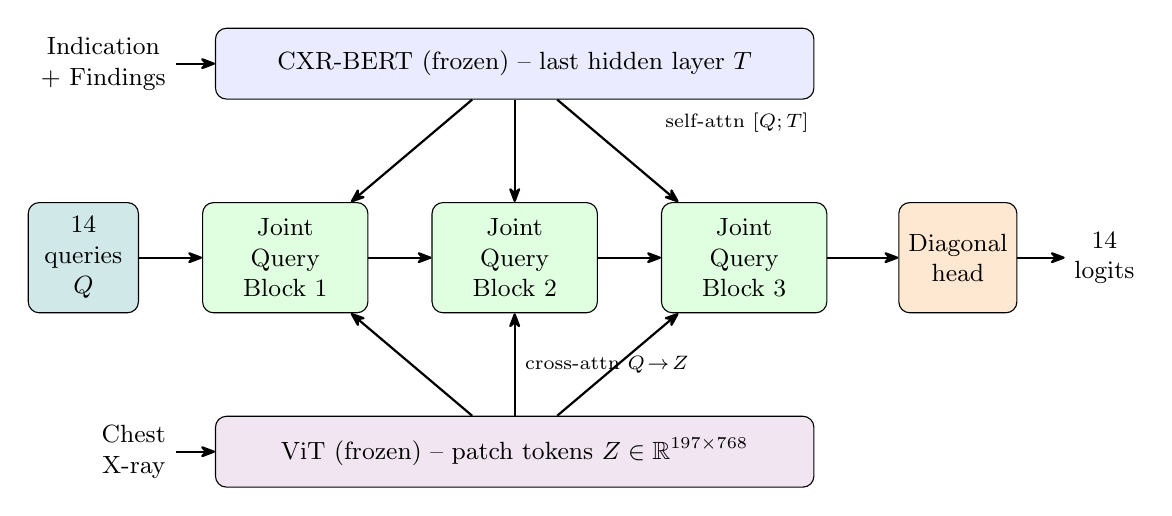
\begin{tikzpicture}[font=\small,>={Stealth[round]},
  enc/.style={draw,rounded corners,fill=blue!8,minimum height=0.9cm,align=center},
  vitst/.style={draw,rounded corners,fill=violet!10,minimum height=0.9cm,align=center},
  blk/.style={draw,rounded corners,fill=green!12,minimum width=2.1cm,minimum height=1.4cm,align=center},
  hd/.style={draw,rounded corners,fill=orange!18,minimum height=1.4cm,minimum width=1.5cm,align=center},
  qy/.style={draw,rounded corners,fill=teal!18,minimum height=1.4cm,minimum width=1.4cm,align=center},
  io/.style={align=center},
  a/.style={->,thick}]
  \node[blk] (b1) {Joint\\Query\\Block 1};
  \node[blk,right=0.8cm of b1] (b2) {Joint\\Query\\Block 2};
  \node[blk,right=0.8cm of b2] (b3) {Joint\\Query\\Block 3};
  \node[qy,left=0.8cm of b1] (q) {$14$\\queries\\$Q$};
  \node[hd,right=0.9cm of b3] (head) {Diagonal\\head};
  \node[io,right=0.6cm of head] (logit) {$14$\\logits};
  \node[enc,above=1.3cm of b2,minimum width=7.6cm] (bert) {CXR-BERT (frozen) -- last hidden layer $T$};
  \node[vitst,below=1.3cm of b2,minimum width=7.6cm] (vit) {ViT (frozen) -- patch tokens $Z\in\mathbb{R}^{197\times768}$};
  \node[io,left=0.5cm of bert.west,anchor=east] (tin) {Indication\\+ Findings};
  \node[io,left=0.5cm of vit.west,anchor=east] (iin) {Chest\\X-ray};
  \draw[a] (q) -- (b1); \draw[a] (b1) -- (b2); \draw[a] (b2) -- (b3);
  \draw[a] (b3) -- (head); \draw[a] (head) -- (logit);
  \draw[a] (tin) -- (bert); \draw[a] (iin) -- (vit);
  \foreach \b in {b1,b2,b3} {\draw[a] (bert) -- (\b);}
  \draw[a] (vit) -- (b1); \draw[a] (vit) -- (b3);
  \draw[a] (vit) -- (b2) node[midway,right,font=\scriptsize]{cross-attn $Q\!\to\!Z$};
  \node[font=\scriptsize,right=0.05cm of bert.south east,anchor=north east,yshift=-0.05cm]{self-attn $[Q;T]$};
\end{tikzpicture}}
\caption{Q-Former \textbf{``last''} variant. Three Joint Query Blocks read the same
final CXR-BERT layer (self-attention over $[Q;T]$) and cross-attend to the frozen ViT
patch tokens; a diagonal head maps each query to its label.}
\label{fig:qf-last}
\end{figure}

\paragraph{``deep'' variant.} Block $k$ reads a \emph{different} CXR-BERT layer
(layers 10, 11, 12 for the three blocks), so the queries integrate text features from
coarse to fine as they go deeper (Figure~\ref{fig:qf-deep}); the image path is
unchanged.

\begin{figure}[H]
\centering
\resizebox{\textwidth}{!}{%
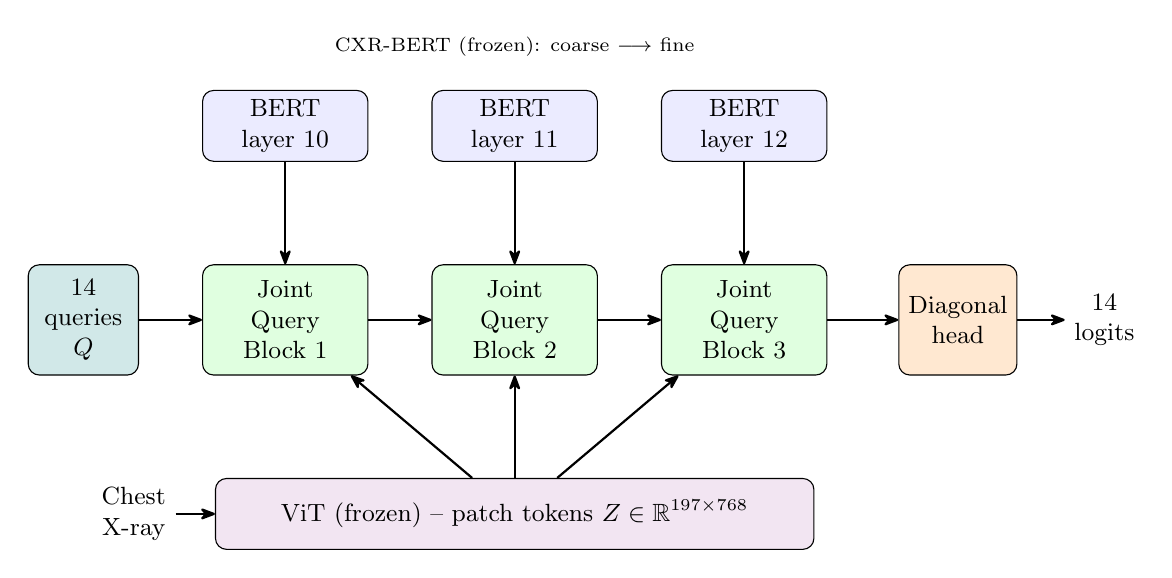
\begin{tikzpicture}[font=\small,>={Stealth[round]},
  enc/.style={draw,rounded corners,fill=blue!8,minimum height=0.9cm,minimum width=2.1cm,align=center},
  vitst/.style={draw,rounded corners,fill=violet!10,minimum height=0.9cm,align=center},
  blk/.style={draw,rounded corners,fill=green!12,minimum width=2.1cm,minimum height=1.4cm,align=center},
  hd/.style={draw,rounded corners,fill=orange!18,minimum height=1.4cm,minimum width=1.5cm,align=center},
  qy/.style={draw,rounded corners,fill=teal!18,minimum height=1.4cm,minimum width=1.4cm,align=center},
  io/.style={align=center},
  a/.style={->,thick}]
  \node[blk] (b1) {Joint\\Query\\Block 1};
  \node[blk,right=0.8cm of b1] (b2) {Joint\\Query\\Block 2};
  \node[blk,right=0.8cm of b2] (b3) {Joint\\Query\\Block 3};
  \node[qy,left=0.8cm of b1] (q) {$14$\\queries\\$Q$};
  \node[hd,right=0.9cm of b3] (head) {Diagonal\\head};
  \node[io,right=0.6cm of head] (logit) {$14$\\logits};
  \node[enc,above=1.3cm of b1] (l10) {BERT\\layer 10};
  \node[enc,above=1.3cm of b2] (l11) {BERT\\layer 11};
  \node[enc,above=1.3cm of b3] (l12) {BERT\\layer 12};
  \node[font=\scriptsize] at ($(l10.north)!0.5!(l12.north)+(0,0.55)$) {CXR-BERT (frozen): coarse $\longrightarrow$ fine};
  \node[vitst,below=1.3cm of b2,minimum width=7.6cm] (vit) {ViT (frozen) -- patch tokens $Z\in\mathbb{R}^{197\times768}$};
  \node[io,left=0.5cm of vit.west,anchor=east] (iin) {Chest\\X-ray};
  \draw[a] (q) -- (b1); \draw[a] (b1) -- (b2); \draw[a] (b2) -- (b3);
  \draw[a] (b3) -- (head); \draw[a] (head) -- (logit);
  \draw[a] (iin) -- (vit);
  \draw[a] (l10) -- (b1); \draw[a] (l11) -- (b2); \draw[a] (l12) -- (b3);
  \draw[a] (vit) -- (b1); \draw[a] (vit) -- (b2); \draw[a] (vit) -- (b3);
\end{tikzpicture}}
\caption{Q-Former \textbf{``deep''} variant. Each Joint Query Block taps a different
CXR-BERT hidden layer (10/11/12), letting the queries fuse text hierarchically; the
frozen ViT path is shared as in the ``last'' variant.}
\label{fig:qf-deep}
\end{figure}

\subsection{Results}

Both variants are trained with the Asymmetric Loss~\cite{asl} and selected on
validation macro AUC. They reach a macro test AUC of \textbf{0.974} (last) and
\textbf{0.978} (deep) -- clearly above the image-only baselines (0.73--0.78,
Section~\ref{sec:cv}) and on par with the strongest text-only model
(Section~\ref{sec:text}). Figures~\ref{fig:qf-last-res} and~\ref{fig:qf-deep-res}
give the per-label breakdown. The fusion therefore \emph{does} add discriminative
power over vision alone; the open question -- as for Architecture~1 -- is how much of
it is genuinely visual.

\begin{figure}[H]
\centering
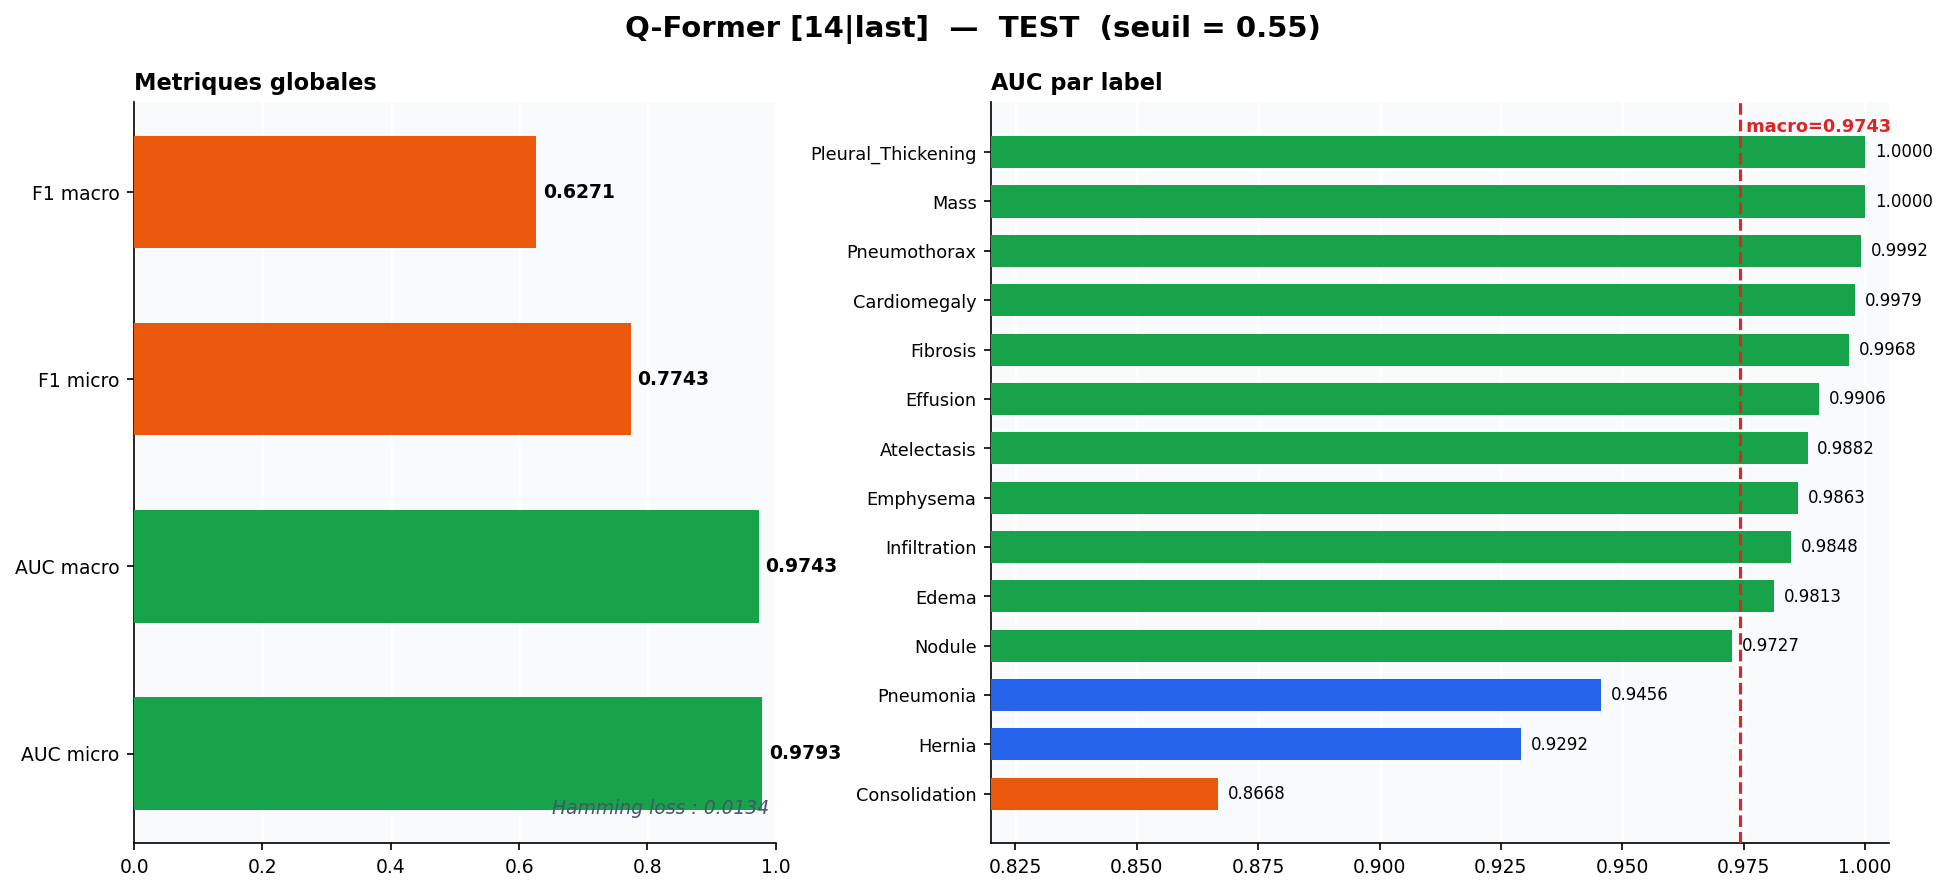
\includegraphics[width=\textwidth]{figures/qformer_last_test.png}
\caption{Q-Former [14$\,|\,$last] -- test metrics and per-label AUC (threshold 0.55).}
\label{fig:qf-last-res}
\end{figure}

\begin{figure}[H]
\centering
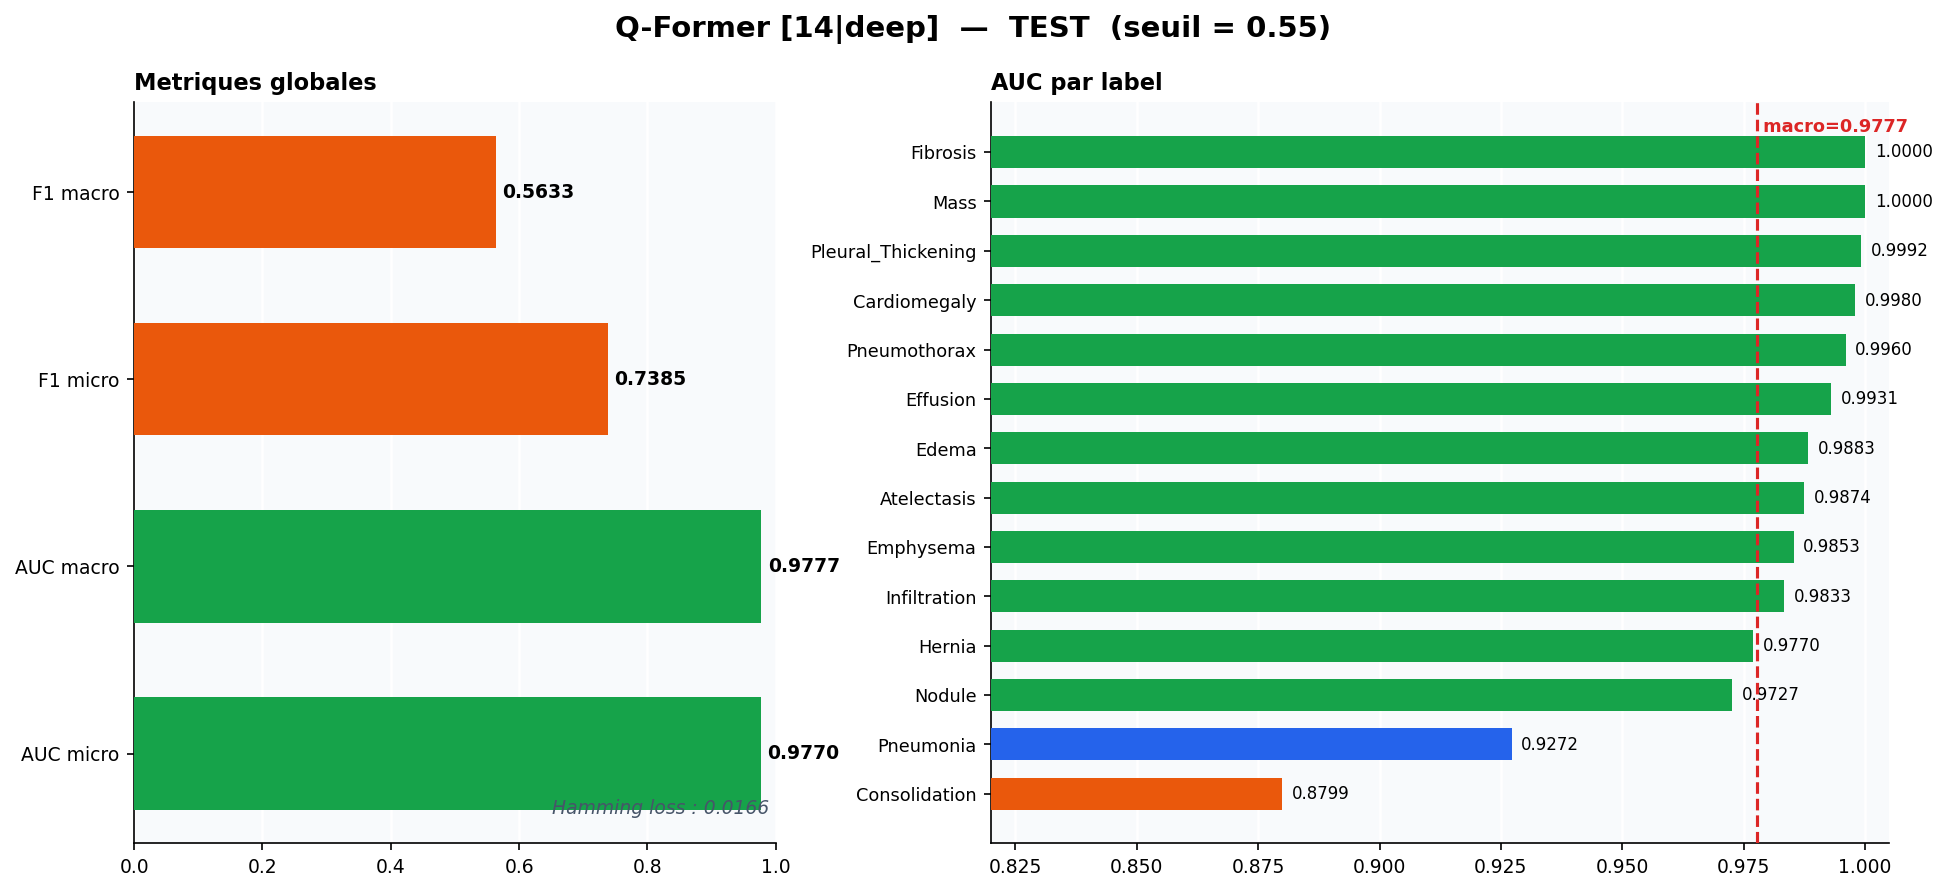
\includegraphics[width=\textwidth]{figures/qformer_deep_test.png}
\caption{Q-Former [14$\,|\,$deep] -- test metrics and per-label AUC (threshold 0.55).}
\label{fig:qf-deep-res}
\end{figure}

\subsection{Explainability and modality balance}
\label{sec:qexplain}

A recurring failure mode of the frozen-encoder Q-Former is \emph{query collapse}: as
depth increases the queries become nearly redundant. Figure~\ref{fig:collapse} shows
the effective rank of the 14 queries dropping from $\sim$13 at initialisation to
$\sim$1.5 after the first block -- i.e.\ the queries stop carrying 14 distinct,
label-specific views and instead converge to a single text-driven direction. This is
the mechanism behind the text dominance: the head reads essentially one fused vector
that is dominated by the (highly predictive) report.

\begin{figure}[H]
\centering
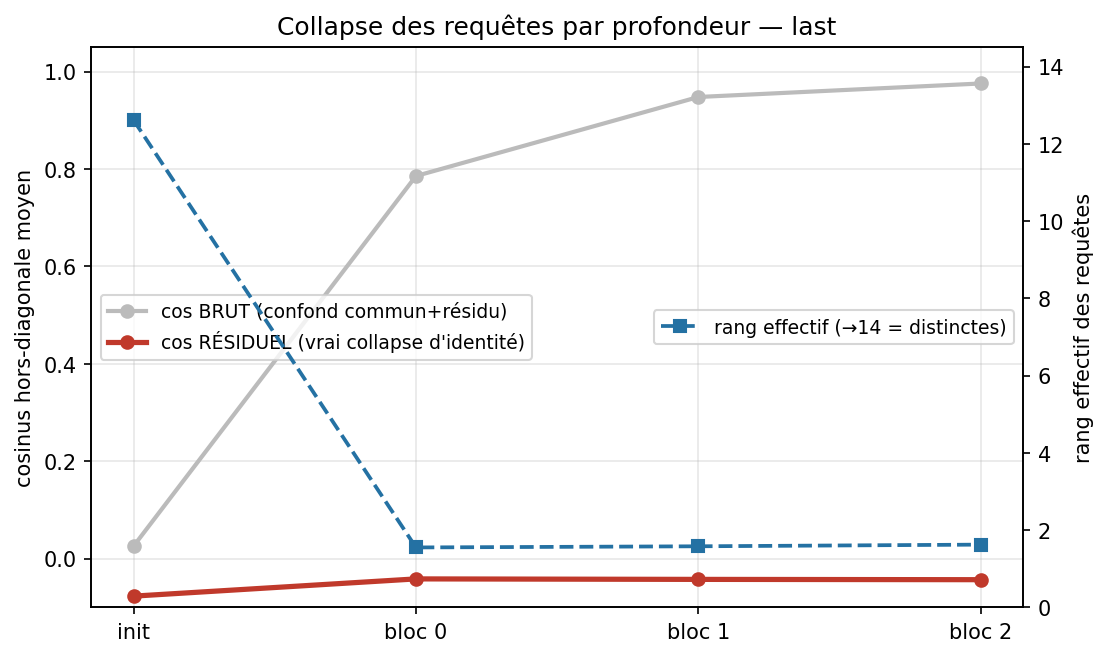
\includegraphics[width=0.7\textwidth]{figures/qformer_collapse.png}
\caption{Query collapse by depth (``last''). Raw inter-query cosine rises while the
effective rank of the query bank falls toward 1, indicating the 14 label queries
collapse onto a single direction.}
\label{fig:collapse}
\end{figure}

We tried several mechanisms to keep the visual channel relevant:
\begin{itemize}
  \item \textbf{Pre-norm} (layer-norm before each sub-layer). This single change is a
        clear \emph{performance jump}: macro AUC \textbf{0.9836} / micro \textbf{0.9870},
        macro F1 \textbf{0.7397} -- our best-performing run -- by stabilising the
        residual stream and partly mitigating collapse.
  \item \textbf{Modality (text) dropout} -- masking the entire text of a fraction
        ($0.3$) of training samples so the queries must occasionally classify from the
        image alone -- combined with pre-norm and identity re-injection. We call this
        configuration \texttt{variant\_c}.
  \item \textbf{Attention-pooled head}, which reads the image through a final
        learned cross-attention so that the attention weights lie \emph{on} the loss
        path (gradients must flow through them); we also used it as a lever against
        label imbalance.
  \item \textbf{CGGM} (contrastive gradient-guided modulation): auxiliary text-only
        and image-only heads, plus a direction loss that pulls the fusion head toward
        whichever modality is improving \emph{slower}, re-balancing the two streams
        during training.
\end{itemize}

The interpretability-oriented \texttt{variant\_c} reaches macro AUC \textbf{0.9795} /
micro \textbf{0.9809} -- a small step below the pre-norm peak -- but its attention is
markedly more localised and label-specific. Figure~\ref{fig:qf-attn} shows the
label-aligned cross-attention of \texttt{variant\_c} on a true \emph{Cardiomegaly}
case: the Cardiomegaly query ($p\!=\!1.00$) concentrates on the cardiac silhouette and
lower mediastinum, while inactive queries (\emph{Edema}, \emph{Mass}) stay diffuse --
the kind of query/label correspondence the diagonal head was designed to expose. The
attention-pooled head pushes interpretability further at a larger accuracy cost
(macro AUC \textbf{0.925}). Table~\ref{tab:qf-variants} summarises the trade-off.

\begin{figure}[H]
\centering
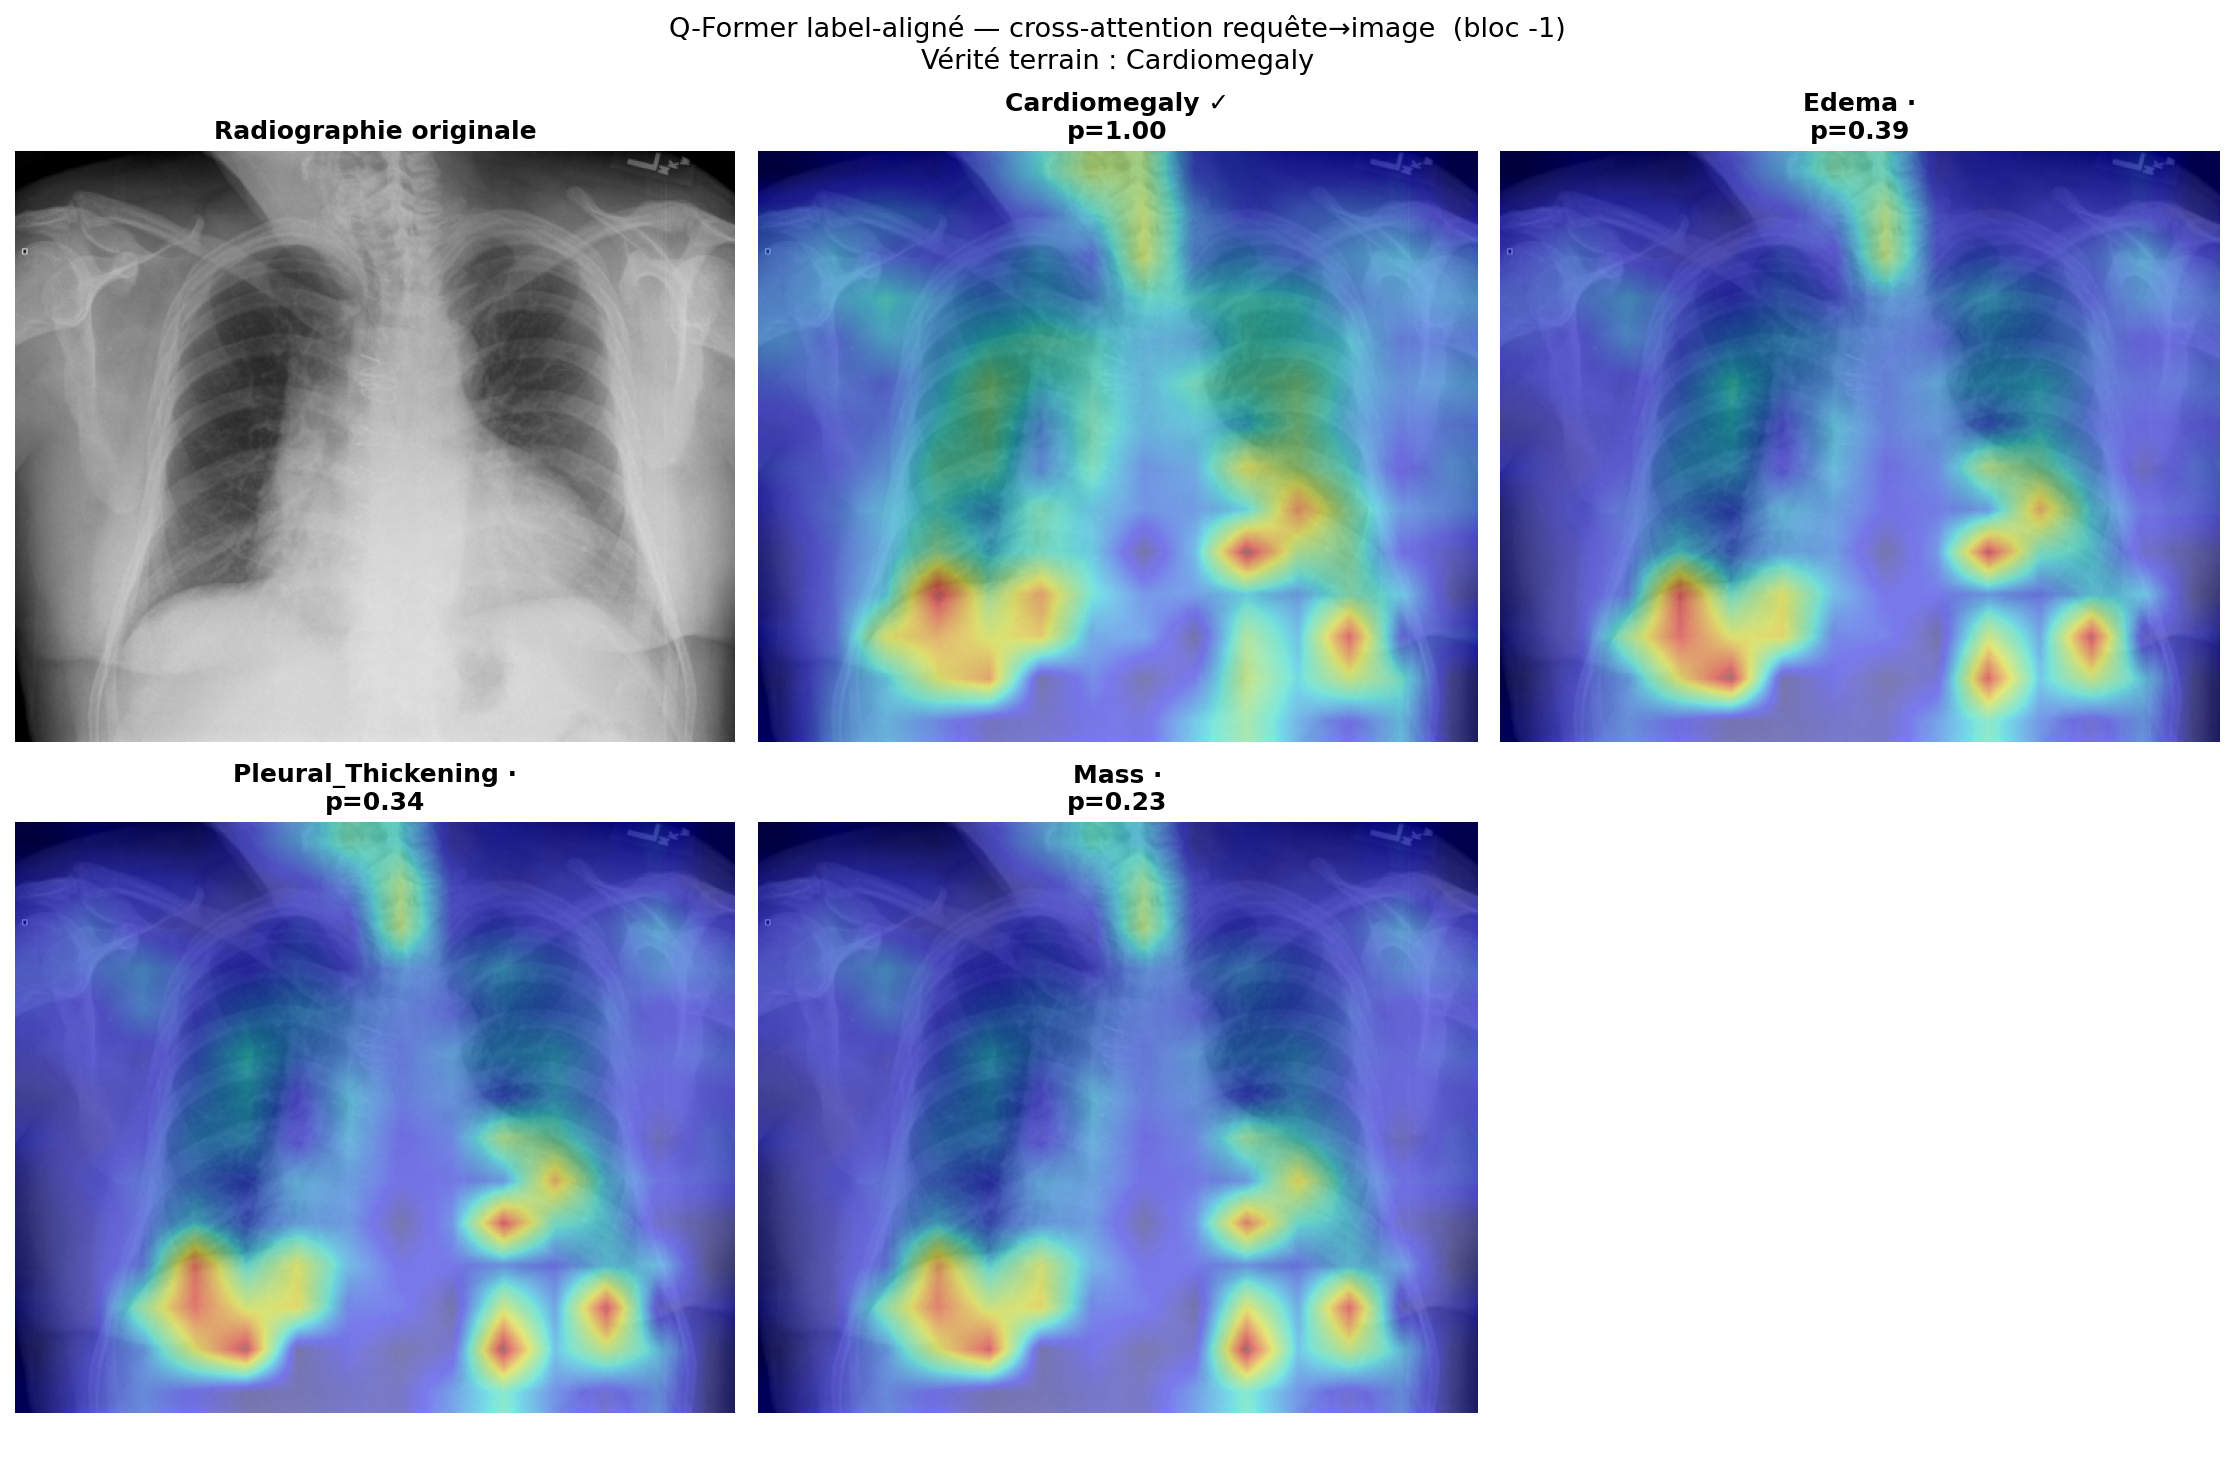
\includegraphics[width=0.92\textwidth]{figures/qformer_variantC_attention.png}
\caption{\texttt{variant\_c} label-aligned cross-attention ($Q\!\to\!Z$) on a
\emph{Cardiomegaly} case. The active Cardiomegaly query localises the cardiac
silhouette; inactive-label queries remain diffuse.}
\label{fig:qf-attn}
\end{figure}

\begin{table}[H]
\centering
\caption{Q-Former variants on the 14-label test set. Pre-norm is the performance
peak; \texttt{variant\_c} and the attention-pooled head trade a little accuracy for
interpretability / modality balance.}
\label{tab:qf-variants}
\begin{tabular}{lccc}
\toprule
Variant & Macro AUC & Micro AUC & Macro F1 \\
\midrule
{[14$\,|\,$last]}                 & 0.9743 & 0.9793 & 0.6271 \\
{[14$\,|\,$deep]}                 & 0.9777 & 0.9770 & 0.5633 \\
Pre-norm (best)                 & \textbf{0.9836} & \textbf{0.9870} & \textbf{0.7397} \\
\texttt{variant\_c} (pre-norm + reinject + text-dropout 0.3) & 0.9795 & 0.9809 & 0.5350 \\
Attention-pooled head           & 0.9246 & 0.9535 & 0.4878 \\
\bottomrule
\end{tabular}
\end{table}

By accepting a $\sim$0.4-point AUC reduction relative to the pre-norm peak,
\texttt{variant\_c} yields a model whose per-label attention is interpretable and
demonstrably less reliant on a single text-driven direction -- the favourable end of
the accuracy/interpretability trade-off for our purposes.

\subsection{In service of unimodality: indication + image only}

Finally, we probed a more clinically realistic setting in which the detailed
\emph{findings} are unavailable at inference and only the short \emph{indication}
accompanies the image (\texttt{--no\_findings}: train on indication + findings, test
on indication + image). Using the deep variant with CGGM and the attention-pooled
head, performance drops sharply -- macro AUC \textbf{0.698}, micro \textbf{0.756},
macro F1 0.123 -- confirming how much of the earlier performance rested on the
findings text. A handful of labels with visible image signatures (\emph{Pneumothorax}
0.875, \emph{Effusion} 0.870, \emph{Cardiomegaly} 0.814) stay well above chance, but
others collapse. These results are not yet conclusive and we report them as
work in progress: forcing the model to lean on the image when the rich report is
withheld is exactly the regime where the interpretability mechanisms above should
matter most.

% ============================================================
\section{Conclusion}
% ============================================================

Across the three modalities the picture is consistent. The \emph{image} alone is a
weak predictor on Open-I (mean AUC 0.73--0.78). The \emph{text} alone is strong: a
TF-IDF + MLP already reaches 0.86 macro AUC and CXR-BERT 0.97, because the
\emph{indication} and \emph{findings} sections frequently state the diagnosis in
words. Multimodal fusion -- whether the symmetric cross-attention of Architecture~1
(0.989 on 21 labels) or the asymmetric Q-Former of Architecture~3 (up to 0.984 on 14
labels) -- improves over the visual baselines, but our interpretability work
(cross-modal mediation, query-collapse analysis, label-aligned attention) shows the
gain is largely \emph{text mediated}. Mechanisms such as pre-norm, modality dropout
(\texttt{variant\_c}), an attention-pooled head, and CGGM let us trade a small amount
of accuracy for a model whose attention is interpretable and whose two streams are
better balanced. The unimodal indication + image setting remains the open problem and
the natural next step, as it directly targets genuine visual reasoning rather than
report paraphrasing.

% ============================================================
\begin{thebibliography}{9}
% ============================================================

\bibitem{openi}
D.~Demner-Fushman \emph{et al.},
``Preparing a collection of radiology examinations for distribution and retrieval,''
\emph{Journal of the American Medical Informatics Association (JAMIA)}, 23(2):304--310, 2016.

\bibitem{transchex}
Project MONAI, ``TransCheX: multimodal (vision + language) transformer for chest X-ray
classification,'' MONAI Research Contributions (software, no associated paper).
\url{https://github.com/Project-MONAI/research-contributions}.

\bibitem{cxrbert}
B.~Boecking \emph{et al.},
``Making the most of text semantics to improve biomedical vision--language processing,''
\emph{European Conference on Computer Vision (ECCV)}, 2022. (BiomedVLP-CXR-BERT.)

\bibitem{blip2}
J.~Li, D.~Li, S.~Savarese, and S.~Hoi,
``BLIP-2: Bootstrapping language-image pre-training with frozen image encoders and large
language models,'' \emph{International Conference on Machine Learning (ICML)}, 2023.

\bibitem{vit}
A.~Dosovitskiy \emph{et al.},
``An image is worth 16$\times$16 words: Transformers for image recognition at scale,''
\emph{International Conference on Learning Representations (ICLR)}, 2021.

\bibitem{asl}
E.~Ben-Baruch \emph{et al.},
``Asymmetric loss for multi-label classification,''
\emph{International Conference on Computer Vision (ICCV)}, 2021.

\end{thebibliography}

\end{document}
